
\begin{question}
Please make a frequency table and a frequency histogram from the
following (sorted) continuous data by rounding to the nearest multiple
of 5.

\begin{longtable}[]{@{}rrrrr@{}}
\toprule
\endhead
39.0865 & 42.1185 & 43.0745 & 48.4095 & 50.4655\tabularnewline
53.6710 & 55.3400 & 57.4980 & 59.9800 & 60.3900\tabularnewline
60.6445 & 62.3565 & 62.8320 & 65.4455 & 65.9020\tabularnewline
66.1680 & 67.1330 & 67.5635 & 68.1090 & 68.9350\tabularnewline
69.1360 & 69.4095 & 69.7555 & 69.8470 & 70.7475\tabularnewline
70.9270 & 71.9800 & 72.1795 & 72.3365 & 74.1170\tabularnewline
\bottomrule
\end{longtable}
\end{question}

\begin{solution}
Make a frequency table.

\begin{longtable}[]{@{}rr@{}}
\toprule
bin & frequency\tabularnewline
\midrule
\endhead
40 & 2\tabularnewline
45 & 1\tabularnewline
50 & 2\tabularnewline
55 & 3\tabularnewline
60 & 4\tabularnewline
65 & 5\tabularnewline
70 & 12\tabularnewline
75 & 1\tabularnewline
\bottomrule
\end{longtable}

Make the histogram.

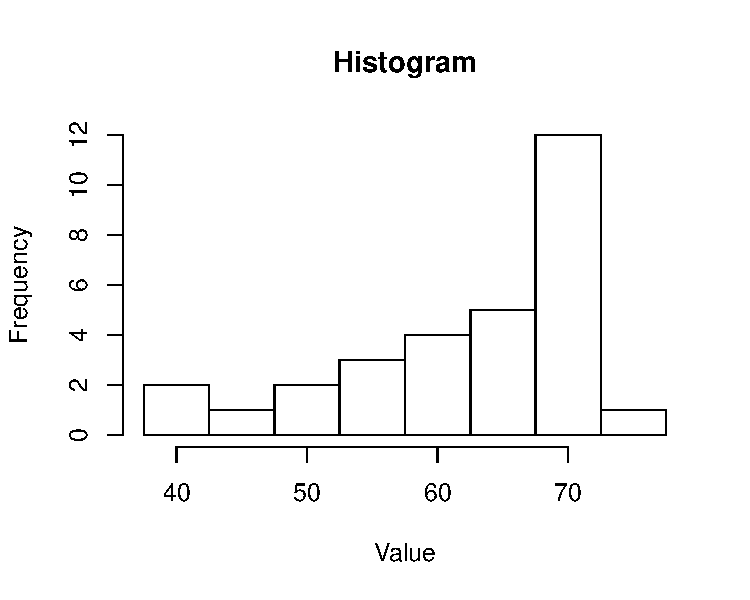
\includegraphics{barchart-1-6.pdf}\\
\end{solution}

